\pagebreak

\begin{itemize}
  \item[\textcolor{white}{$\Box$}] 
\end{itemize}


\vspace{7cm}

\begin{figure}[H]
  
\includegraphics{Images/part_iii.png}
\end{figure}

\section*{}
\addcontentsline{toc}{section}{PARTIE II: ETUDES PRATIQUES}

\pagebreak


\setcounter{section}{0} % Restart the section counter
\section{INTRODUCTION}

Cette partie est la plus fondamentale de cette thèse. Elle est d’une grande importance car elle fournit des informations détaillées sur les protocoles et les outils déployés pour mener à bien notre étude sur l’acceptabilité de la contraception injectable au sein des établissements de santé, particulièrement du point de vue des professionnels de la santé. \\

\noindent Dans les pages qui suivent, nous détaillerons les éléments fondamentaux utilisés pour recueillir, analyser et interpréter les données issues de l’enquête menée auprès des professionnels de la santé via un questionnaire. \\    

\noindent Ces informations ont pour but de fournir une vue d’ensemble de notre démarche, ce qui permettra de suivre le cheminement qui nous a conduits aux résultats que nous allons présenter. Elles garantissent également la transparence de notre travail.

\section{METHODOLOGIE ET RESULTATS }
\subsection{Matériels}
\subsubsection{Objectifs de l’étude : }

\begin{itemize}
  \item Objectif général : \\
  L’objectif général de cette étude consiste à évaluer l’acceptabilité de la contraception injectable au sein des établissements de santé publique auprès des professionnels de santé.  
  \item Objectifs spécifiques :  
  \begin{itemize}[label={$\circ$}, nosep]
    \item Identifier les facteurs influençant l’acceptabilité de la contraception injectable. 
    \item Formuler des recommandations visant à améliorer l’acceptabilité de la contraception injectable, en prenant en compte les résultats de l’étude.  
    \end{itemize}
\end{itemize}

\subsubsection{Type d’étude : }

Il s’agit d’une étude descriptive et rétrospective. 

\subsubsection{Lieux et période de recueil des données : }

La collecte des données s'est déroulée au sein des centres de santé publique de Rabat, Salé, Kénitra et Témara, sur une période s'étalant d'août à septembre 2023.

\subsubsection{Population}

\subsubsubsection{Critères d’inclusion : }
Les critères d’inclusions étaient : 
\begin{itemize}
  \item Les professionnels de santé travaillant dans des établissements de santé publique,  
  \item Les professionnels de santé ayant des connaissances et de l’expérience dans le domaine de la contraception, en particulier la contraception injectable. 
\end{itemize}

\subsubsection{Critères de non inclusion : }
Les critères de non inclusion étaient : 

\begin{itemize}
  \item	Les professionnels de santé travaillant dans le secteur privé, 
  \item Les professionnels de santé n’ayant pas d’expérience en matière de contraception, 
  \item Les professionnels de santé ne désirant pas participer à l’étude, 
  \item Les professionnels de santé n’ayant pas répondu à la totalité des questions de l’enquête,
  \item	Les membres du grand public.
\end{itemize}

\subsection{Méthodologie }

\subsubsection{Outils de l’enquête :}

Un questionnaire créé avec l’outil Google Forms.

\subsubsection{Méthode de recueil des données :}
L’ensemble des données a été recueilli par l’auto remplissage du questionnaire par les professionnels de santé eux-mêmes.   

\subsubsection{Traitement et analyse des données :}

La saisie et l’analyse des données ont été faites sur Microsoft Word et Microsoft Excel.  

\subsubsection{Méthode de recherche bibliographique : }

Les articles pertinents ont été tirés de ScienceDirect, Google Scholar et PubMed pour la recherche bibliographique et le logiciel Zotero a permis de les citer.

\subsection{Résultats de l’étude : }

44 questionnaires ont étés remplis, dont 4 ont été mal remplis et 40 correctement remplis. 

\iffalse
\begin{table}[htbp]
\centering
\renewcommand{\arraystretch}{1.5}
  \begin{spacing}{1.5}
\arrayrulecolor{blue} % Set the color of the border lines to blue
\begin{tabular}{|>{\bfseries}l|l|l|}
    \hline
    \rowcolor{blue!20} % Set the background color of the first row to blue!20
    \textcolor{Statuts professionnel } & \textcolor{Effectif} & \textcolor{Pourcentage} \\
    \hline(x, y)
    Infirmier & 9 & 22,50\% \\
    \hline
    Sage-femme & 14 & 35\% \\
    \hline
    Médecin & 17 & 42,50\% \\
    \hline
    Total & 40 & 100\% \\
    \hline
\end{tabular}
\end{spacing}
\caption{Example table with blue border lines and a blue background in the first row}
\label{tab:blue_border_lines}
\end{table}
\fi

\begin{table}[H]
  \centering
  \renewcommand{\arraystretch}{1.5}
  \arrayrulecolor{customcolor!90}
  \caption{Répartition en fonction du statut professionnel}
  \begin{spacing}{1.5} % Set line spacing to 1.5
  \begin{tabularx}{\textwidth}{|X|X|X|}
      \hline
      \rowcolor{customcolor!90}
      \textbf{\color{white}Statuts professionnel} & \textbf{\color{white}Effectif} & \textbf{\color{white}Pourcentage}  \\
      \hline
      Infirmier & 9  & 22,50\% \\
      \hline
      Sage-femme & 14 & 35\% \\
      \hline
      Médecin & 17 & 42,50\% \\
     \hline
      Total & 40 & 100\% \\
      \hline
  \end{tabularx}
\end{spacing}

  %\label{tab:my_table}
\end{table}

\noindent La majorité des participants à cette étude étaient des médecins, soit 42,50\%.  

\begin{figure}[H]
  \centering
  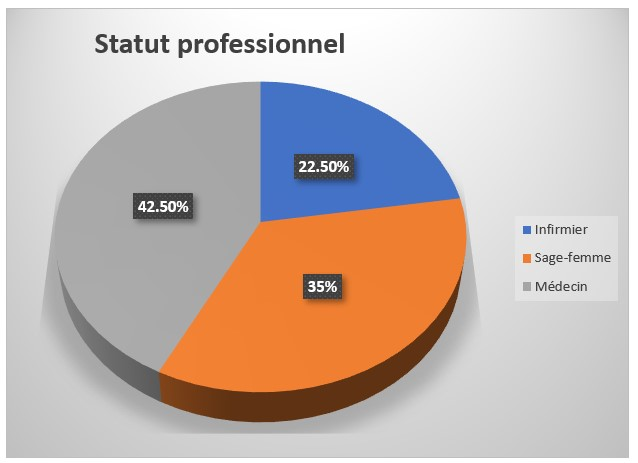
\includegraphics{Images/fig_45.jpg}
  \caption{La majorité des participants à cette étude étaient des médecins, soit 42,50\%. }
  
\end{figure}

\begin{table}[H]
  \centering
  \renewcommand{\arraystretch}{1.5}
  \arrayrulecolor{customcolor!90}
  \caption{Répartition en fonction du statut professionnel}
  \begin{spacing}{1.5} % Set line spacing to 1.5
  \begin{tabularx}{\textwidth}{|X|X|X|}
      \hline
      \rowcolor{customcolor!90}
      \textbf{\color{white}Lieu d’exercice} & \textbf{\color{white}Effectif} & \textbf{\color{white}Pourcentage}  \\
      \hline
      Centre de santé & 40  & 100\% \\
      \hline
      Dispensaire & 0 & 0\% \\
      \hline
      Centre mère-enfant & 0 & 0\% \\
      \hline
      Hôpital régional & 0 & 0\% \\
      \hline
      Hôpital provincial & 0 & 0\% \\
      \hline
      CHU & 0 & 0\% \\
     \hline
      Total & 40 & 100\% \\
      \hline
  \end{tabularx}
\end{spacing}

  %\label{tab:my_table}
\end{table}

\noindent Cette étude a été réalisée exclusivement dans les centres de santé. 

\begin{figure}[H]
  \centering
  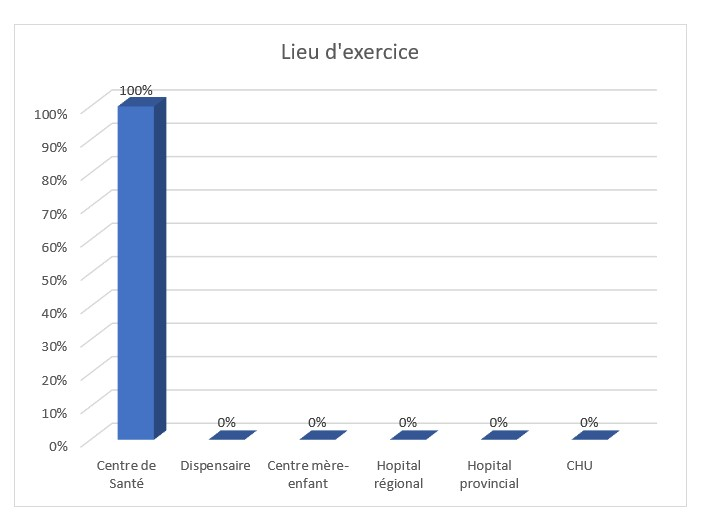
\includegraphics[scale=1.2]{Images/fig_46.jpg}
  \caption{Répartition en fonction du lieu d’exercice}
  
\end{figure}

\begin{table}[H]
  \centering
  \renewcommand{\arraystretch}{1.5}
  \arrayrulecolor{customcolor!90}
  \caption{Zone d’exercice}
  \begin{spacing}{1.5} % Set line spacing to 1.5
  \begin{tabularx}{\textwidth}{|X|X|X|}
      \hline
      \rowcolor{customcolor!90}
      \textbf{\color{white}Zone d’exercice} & \textbf{\color{white}Effectif} & \textbf{\color{white}Pourcentage}  \\
      \hline
      Zone urbaine & 39 & 97,50\% \\
      \hline
      Zone rurale & 1 & 2,50\% \\
     \hline
      Total & 40 & 100\% \\
      \hline
  \end{tabularx}
\end{spacing}

  %\label{tab:my_table}
\end{table}

\noindent L’étude a été réalisée principalement dans les zones urbaines, soit 97,50\%. 

\begin{figure}[H]
  \centering
  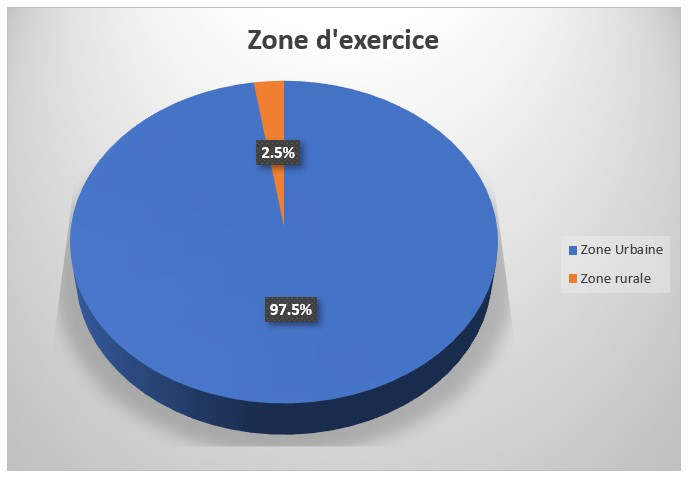
\includegraphics{Images/fig_47.jpg}
  \caption{Zone d’exercice}  
\end{figure}

\begin{table}[H]
  \centering
  \renewcommand{\arraystretch}{1.5}
  \arrayrulecolor{customcolor!90}
  \caption{Méthodes contraceptives les plus prescrites}
  \begin{spacing}{1.5} % Set line spacing to 1.5
  \begin{tabularx}{\textwidth}{|p{8cm}|X|X|}
      \hline
      \rowcolor{customcolor!90}
      \textbf{\color{white}Méthodes contraceptives} & \textbf{\color{white}Effectif} & \textbf{\color{white}Pourcentage}  \\
      \hline
      Contraception orale & 37 & 92,50\% \\
      \hline
      Contraception orale et contraception \newline injectable & 2 & 5\% \\
      \hline
      Préservatifs  & 1 & 2,5\% \\
      \hline
      Contraception injectable & 0 & 0\% \\
     \hline
      Total & 40 & 100\% \\
      \hline
  \end{tabularx}
\end{spacing}

  %\label{tab:my_table}
\end{table}

\noindent La méthode contraceptive la prescrite est la contraception orale (92,50\%).

\begin{figure}[H]
  \centering
  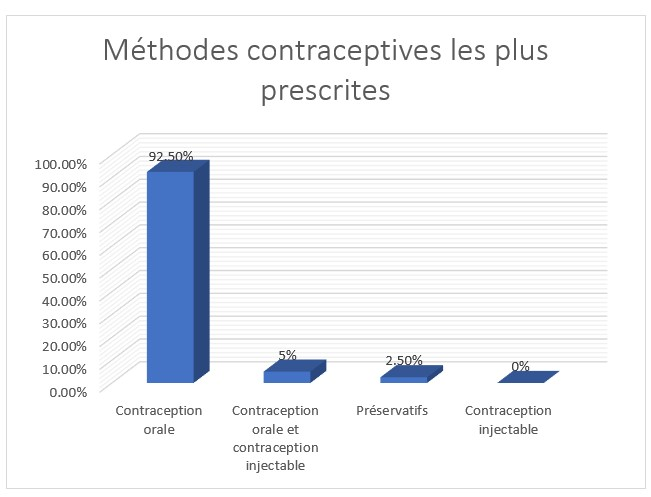
\includegraphics[scale=1.23]{Images/fig_48.jpg}
  \caption{Méthodes contraceptives les plus prescrites}
\end{figure}

\begin{table}[H]
  \centering
  \renewcommand{\arraystretch}{1.5}
  \arrayrulecolor{customcolor}
  \caption{Suggestion de la contraception injectable}
  \begin{spacing}{1.5} % Set line spacing to 1.5
  \begin{tabularx}{\textwidth}{|X|X|X|}
      \hline
      \rowcolor{customcolor!90}
      \textbf{\color{white}Suggestion de la \newline contraception injectable} & \textbf{\color{white}Effectif} & \textbf{\color{white}Pourcentage}  \\
      \hline
      Oui & 33 & 82,50\% \\
      \hline
      Non & 7 & 17,50\% \\
     \hline
      Total & 40 & 100\% \\
      \hline
  \end{tabularx}
\end{spacing}

  %\label{tab:my_table}
\end{table}

\noindent La majorité des professionnels de santé, soit 82,50\%, ont proposé la contraception injectable aux femmes. 

\begin{figure}[H]
  \centering
  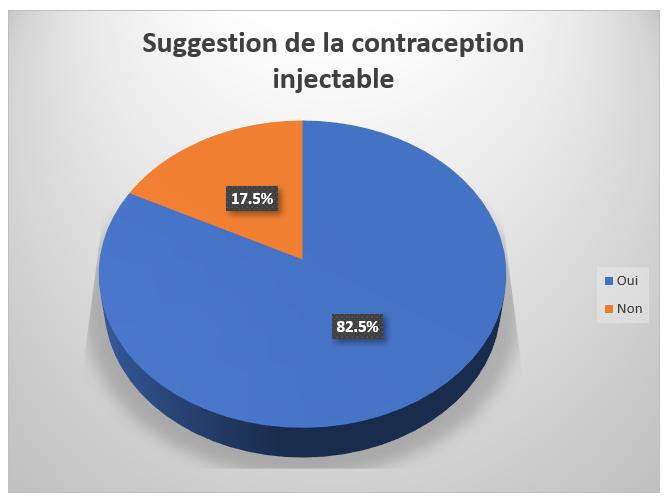
\includegraphics{Images/fig_49.png}
  \caption{Suggestion de la contraception injectable}
  
\end{figure}

\begin{table}[H]
  \centering
  \renewcommand{\arraystretch}{1.5}
  \arrayrulecolor{customcolor}
  \caption{Suggestion de la contraception injectable}
  \begin{spacing}{1.5} % Set line spacing to 1.5
  \begin{tabularx}{\textwidth}{|p{8cm}|X|X|}
      \hline
      \rowcolor{customcolor}
      \textbf{\color{white}Avantages de la contraception  \newline injectable} & \textbf{\color{white}Effectif} & \textbf{\color{white}Pourcentage}  \\
      \hline
      Surmonte l’oubli & 35 & 87,50\% \\
      \hline
      Longue durée de contraception & 32 & 80\% \\
      \hline
      Moins d’effets indésirables & 8 & 20\% \\
      \hline
  \end{tabularx}
\end{spacing}

  %\label{tab:my_table}
\end{table}

\noindent NB : Une personne peut donner plusieurs réponses

\vspace{2em}

\noindent Les principaux avantages de la contraception injectable selon cette étude sont de surmonter l’oubli (87,50) et d’assurer une contraception à long terme (80\%). 


\begin{figure}[H]
  \centering
  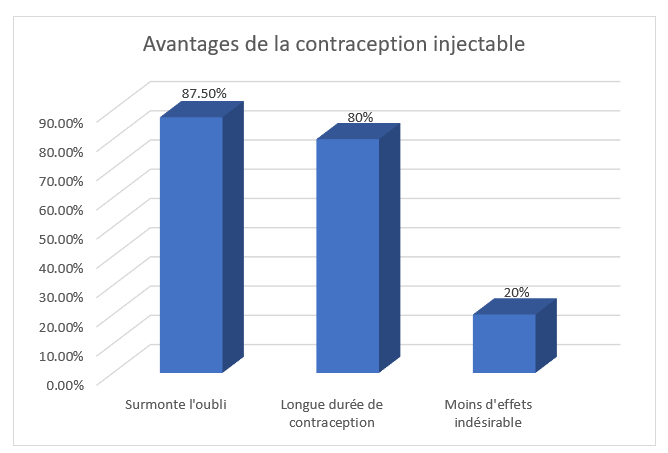
\includegraphics[scale=1.23]{Images/fig_50.png}
  \caption{Avantages de la contraception injectable}
\end{figure}

\begin{table}[H]
  \centering
  \renewcommand{\arraystretch}{1.5}
  \arrayrulecolor{customcolor}
  \caption{Inconvénients de la contraception injectable}
  \begin{spacing}{1.5} % Set line spacing to 1.5
  \begin{tabularx}{\textwidth}{|p{8cm}|X|X|}
      \hline
      \rowcolor{customcolor}
      \textbf{\color{white}Inconvénients \hspace{1cm} de \,\, la  \newline contraception injectable} & \textbf{\color{white}Effectif} & \textbf{\color{white}Pourcentage}  \\
      \hline
      Plus d’effets indésirables & 22 & 55\% \\
      \hline
      Irréversible dans la durée prescrite  & 15 & 37,50\% \\
      \hline
      Risque \,\,\, d’infection \,\, du \,\, site \newline d’administration & 6 & 15\% \\
      \hline
      Pas d’inconvénients & 3 & 7,50\% \\
      \hline
      Arthrose & 1 & 2,50\% \\
      \hline
      Pas d’inconvénients si les contre-indications sont respectées & 1 & 2,50\% \\
      \hline
  \end{tabularx}
\end{spacing}

  %\label{tab:my_table}
\end{table}

\noindent NB : Une personne peut donner plusieurs réponses

\vspace{2em}

\noindent Les principaux inconvénients de cette méthode selon l’étude sont ses effets indésirables (55\%) et son irréversibilité dans la durée prescrite (37,50\%). 

\begin{figure}[H]
  \centering
  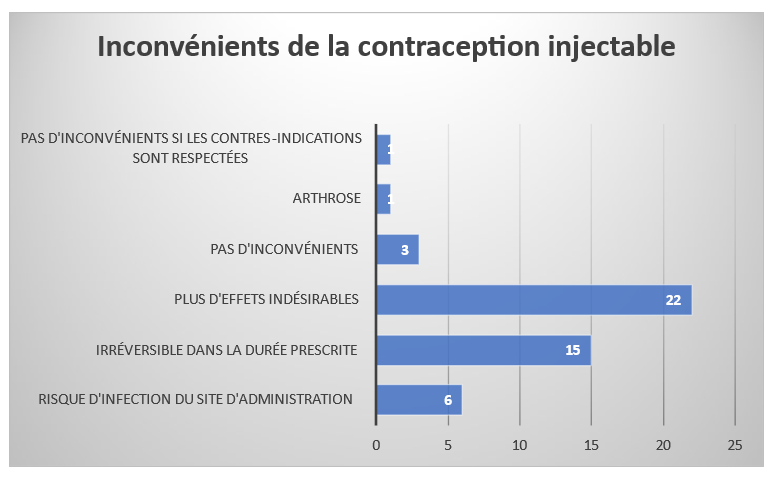
\includegraphics[scale=1.1]{Images/fig_51.png}
  \caption{Avantages de la contraception injectable}  
\end{figure}

\begin{table}[H]
  \centering
  \renewcommand{\arraystretch}{1.5}
  \arrayrulecolor{customcolor}
  \caption{Inconvénients de la contraception injectable}
  \begin{spacing}{1.5} % Set line spacing to 1.5
  \begin{tabularx}{\textwidth}{|p{8cm}|X|X|}
      \hline
      \rowcolor{customcolor}
      \textbf{\color{white}Acceptabilité \hspace{1cm} de \,\, la  \newline contraception injection} & \textbf{\color{white}Effectif} & \textbf{\color{white}Pourcentage}  \\
      \hline
      Très acceptable & 4 & 10\% \\
      \hline
      Peu acceptable  & 31 & 77,50\% \\
      \hline
      Non acceptable & 5 & 12,5\% \\
      \hline
      Total & 40 & 100\% \\
      
      \hline
  \end{tabularx}
\end{spacing}

  %\label{tab:my_table}
\end{table}

\noindent Cette méthode contraceptive est majoritairement peu acceptable, soit 77,50\%. 

\begin{figure}[H]
  \centering
  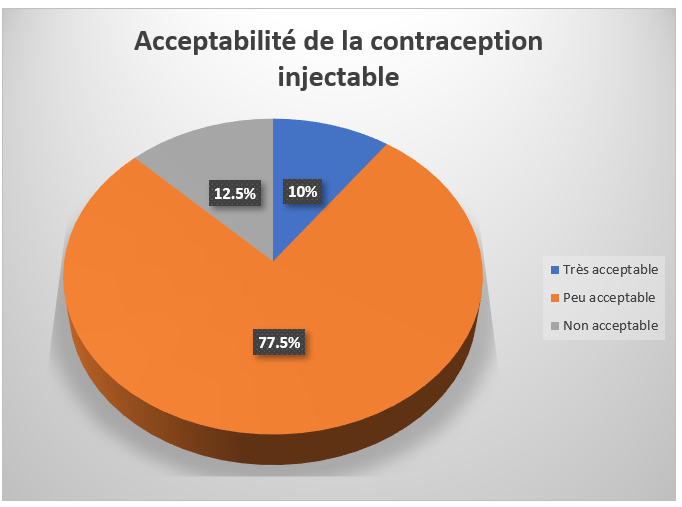
\includegraphics[scale=1]{Images/fig_52.png}
  \caption{Acceptabilité de la contraception injectable}
   
\end{figure}

\begin{table}[H]
  \centering
  \renewcommand{\arraystretch}{1.5}
  \arrayrulecolor{customcolor}
  \caption{Inconvénients de la contraception injectable}
  \begin{spacing}{1.5} % Set line spacing to 1.5
  \begin{tabularx}{\textwidth}{|p{8cm}|X|X|}
      \hline
      \rowcolor{customcolor}
      \textbf{\color{white}Adhérence à la contraception injectable} & \textbf{\color{white}Effectif} & \textbf{\color{white}Pourcentage}  \\
      \hline
       Oui & 31 & 77,50\% \\
      \hline
      Non  & 9 & 2,50\% \\
      \hline  
      Total & 40 & 100\% \\
      
      \hline
  \end{tabularx}
\end{spacing}

  %\label{tab:my_table}
\end{table}

\noindent La plupart des utilisatrices adhère à cette méthode contraceptive, soit 77,50\%. 

\begin{figure}[H]
  \centering
  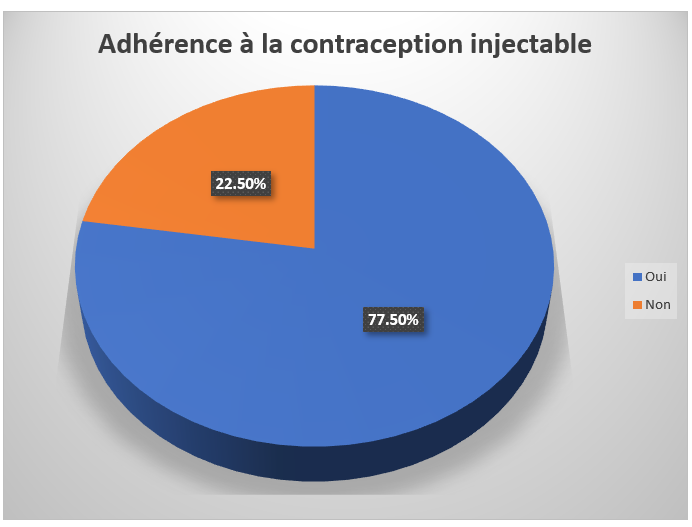
\includegraphics{Images/fig_53.png}
  \caption{Adhérence à la contraception injectable}
  
\end{figure}

\begin{table}[H]
  \centering
  \renewcommand{\arraystretch}{1.5}
  \arrayrulecolor{customcolor}
  \caption{Effets indésirables signalés par les utilisatrices}
  \begin{spacing}{1.5} % Set line spacing to 1.5
  \begin{tabularx}{\textwidth}{|p{8cm}|X|X|}
      \hline
      \rowcolor{customcolor}
      \textbf{\color{white}Effets indésirables signalés \newline par les utilisatrices} & \textbf{\color{white}Effectif} & \textbf{\color{white}Pourcentage}  \\
      \hline
      Troubles menstruels & 34 & 85\% \\
      \hline
      Prise de poids   & 23 & 57,50\% \\
      \hline
      Baisse de la libido & 6 & 15\% \\
      \hline
      Réaction au site d’injection & 6 & 15\% \\
      \hline
      Hypersensibilité mammaire & 3 & 7,50\% \\
      \hline
      Hirsutisme (la pilosité) & 2 & 5\% \\
      \hline
      Varices & 1 & 2,50\% \\
      
      \hline
  \end{tabularx}
\end{spacing}

  %\label{tab:my_table}
\end{table}

\noindent NB : Une personne peut donner plusieurs réponses

\vspace{2em}

\noindent Les principaux effets indésirables signalés par les utilisatrices sont les troubles menstruels, soit 85\% et la prise de poids, soit 57,50\%. 

\begin{figure}[H]
  \centering
  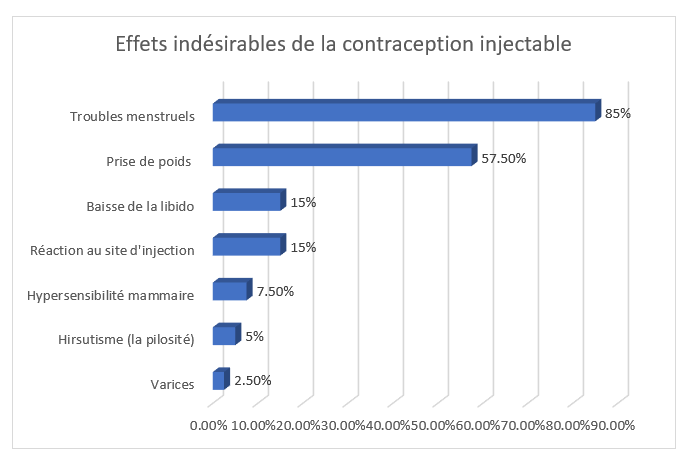
\includegraphics[scale=1.15]{Images/fig_54.png}
  \caption{Effets indésirables signalés par les patients}
  
\end{figure}

\begin{table}[H]
  \centering
  \renewcommand{\arraystretch}{1.5}
  \arrayrulecolor{customcolor}
  \caption{Cas d’échecs de la contraception injectable}
  \begin{spacing}{1.5} % Set line spacing to 1.5
  \begin{tabularx}{\textwidth}{|p{8cm}|X|X|}
      \hline
      \rowcolor{customcolor}
      \textbf{\color{white}Cas d’échec \,\, de \,\, la contraception \newline injectable} & \textbf{\color{white}Effectif} & \textbf{\color{white}Pourcentage}  \\
      \hline
      Oui & 3 & 7,50\% \\
      \hline
      Non  & 37 & 92,50\% \\
      \hline
      Total & 40 & 100\% \\
      
      \hline
  \end{tabularx}
\end{spacing}

  %\label{tab:my_table}
\end{table}

\noindent La contraception injectable est efficace avec des cas d’échec minimes, soit 7,50\%. 

\begin{figure}[H]
  \centering
  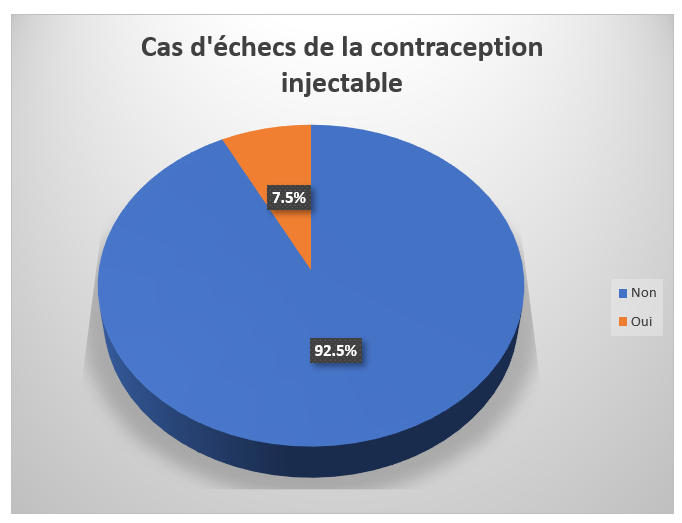
\includegraphics[scale=1.1]{Images/fig_55.png}
  \caption{Cas d’échecs de la contraception injectable}
  
\end{figure}

\begin{table}[H]
  \centering
  \renewcommand{\arraystretch}{1.5}
  \arrayrulecolor{customcolor}
  \caption{Potentielles causes d’échecs}
  \begin{spacing}{1.5} % Set line spacing to 1.5
  \begin{tabularx}{\textwidth}{|p{8cm}|X|X|}
      \hline
      \rowcolor{customcolor}
      \textbf{\color{white}Potentielles causes d’échec} & \textbf{\color{white}Effectif} & \textbf{\color{white}Pourcentage}  \\
      \hline
      Tolérance& 2 & 50\% \\
      \hline
      Non-respect du délai d’abstinence  & 1 & 25\% \\
      \hline
      Enceinte avant de prendre & 1 & 25\% \\
      
      \hline
  \end{tabularx}
\end{spacing}

  %\label{tab:my_table}
\end{table}

\begin{figure}[H]
  \centering
  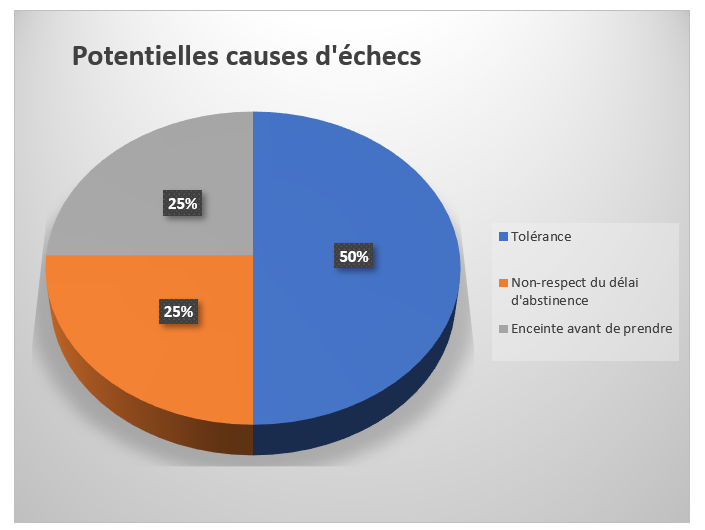
\includegraphics[scale=1.1]{Images/fig_56.jpg}
  \caption{Potentielles causes d’échecs}
  
\end{figure}


\begin{table}[H]
  \centering
  \renewcommand{\arraystretch}{1.5}
  \arrayrulecolor{customcolor}
  \caption{Suivi pour les patientes}
  \begin{spacing}{1.5} % Set line spacing to 1.5
  \begin{tabularx}{\textwidth}{|p{8cm}|X|X|}
      \hline
      \rowcolor{customcolor}
      \textbf{\color{white}Suivi pour les utilisatrices \newline sous contraception injectable} & \textbf{\color{white}Effectif} & \textbf{\color{white}Pourcentage}  \\
      \hline
      Oui & 38 & 95\% \\
      \hline
      Non  & 2 & 5\% \\
      \hline
      Total & 40 & 100\% \\
      
      \hline
  \end{tabularx}
\end{spacing}

  %\label{tab:my_table}
\end{table}

\noindent La plupart des utilisatrices de cette méthode contraceptive sont suivies, soit 95\%. 

\begin{figure}[H]
  \centering
  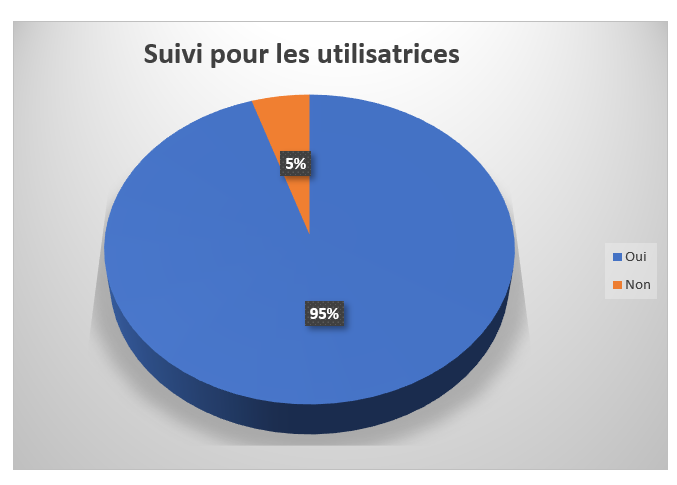
\includegraphics[scale=1.1]{Images/fig_57.png}
  \caption{Suivi pour les utilisatrices}
  
\end{figure}


\begin{table}[H]
  \centering
  \renewcommand{\arraystretch}{1.5}
  \arrayrulecolor{customcolor}
  \caption{Degrés de satisfaction}
  \begin{spacing}{1.5} % Set line spacing to 1.5
  \begin{tabularx}{\textwidth}{|p{8cm}|X|X|}
      \hline
      \rowcolor{customcolor}
      \textbf{\color{white}Degrés de satisfaction des utilisatrices} & \textbf{\color{white}Effectif} & \textbf{\color{white}Pourcentage}  \\
      \hline
      Satisfaites & 24 & 60\% \\
      \hline
      Peu satisfaites  & 13 & 32,50\% \\
      \hline
      Non satisfaites & 3 & 7,50\% \\
      \hline
      Total & 40 & 100\% \\
      
      \hline
  \end{tabularx}
\end{spacing}

  %\label{tab:my_table}
\end{table}


\noindent Selon l’étude, plus de la moitié des utilisatrices de cette méthode contraceptive sont satisfaites, soit 60\%. 

\begin{figure}[H]
  \centering
  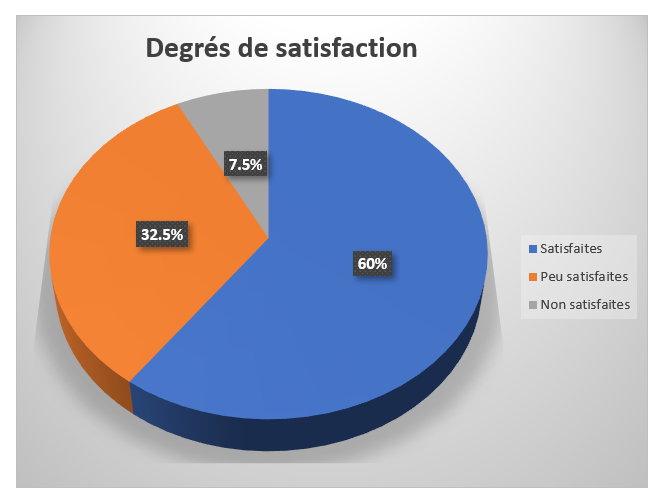
\includegraphics[scale=1.1]{Images/fig_58.png}
  \caption{Degrés de satisfaction}
  
\end{figure}


\section{ANALYSES ET DISCUSSIONS  }

\subsection{Population étudiée :}

L’étude a été menée auprès de différents professionnels de la santé impliqués dans la prescription et le conseil en matière de la contraception pour les femmes. Ces professionnels de santé jouent un rôle crucial en guidant les femmes dans leur choix, en expliquant les avantages, les inconvénients, les effets secondaires et en assurant leur suivi. (101) \\

\noindent La majorité de la population qui a participé à cette étude était composée de médecins (42,50\%), suivis par les sage-femmes (35\%) et les infirmiers (22,50\%). 

\subsection{Lieu d’exercice :}

\noindent L'ensemble de notre étude s'est déroulé exclusivement au sein des centres de santé, en raison de leur rôle central dans la mise en œuvre des services de planification familiale dans le secteur public.\\

\noindent Cette décision s'appuie sur les normes établies par le ministère de la Santé, comme documenté dans les standards des méthodes de planification familiale au Maroc. Selon ce document, à l'exception de la stérilisation qui doit être réalisée à l'hôpital, tous les autres moyens de contraception sont principalement accessibles au sein des centres de santé. (4) \\

\noindent Une étude réalisée en Ouganda en 2022 portant sur l’auto-injection de contraceptifs à travers la prestation régulière de services auprès des professionnels de santé dans le secteur public par Morozoff et al. a été réalisée exclusivement, soit 100\% dans les centres de santé,  ce qui valide notre conclusion soulignant ainsi que les services de contraception sont principalement obtenus dans les centres de santé. (102)\\

\noindent Notre résultat est également cohérent avec une étude menée au Mali en 2023 par DOLO M., qui a porté sur les connaissances, attitudes et pratiques des jeunes en matière de contraception moderne. Dans cette étude, les centres de santé étaient également identifiés comme le lieu privilégié d'approvisionnement en produits contraceptifs, cités par 85\% des participants. (103) \\


\begin{table}[H]
  \centering
  \renewcommand{\arraystretch}{1.5}
  \arrayrulecolor{black}

  \begin{spacing}{1.5} % Set line spacing to 1.5
  \begin{tabularx}{\textwidth}{|X|X|X|X|}
      \hline
      % \rowcolor{customcolor}
      \textbf{Lieu d’exercice} & \textbf{Notre étude } & \textbf{Morozoff et al.} & \textbf{DOLO M.} \\
      \hline
      Centre de santé & 100\% & 100\% & 85\% \\
      
      
      \hline
  \end{tabularx}
\end{spacing}
\captionsetup{justification=centering} % Center-align the caption
\caption{Comparaison de notre étude avec d’autres études sur le lieu d’exercice des \hspace{2cm} professionnels de santé}

  %\label{tab:my_table}
\end{table}

\subsection{Zone d’exercice :}

L’étude a été réalisée principalement dans les zones urbaines 97,50\% parce qu’elles étaient plus accessibles. Elle a également été réalisée dans des zones rurales, soit 2,50\%.    

\subsection{Méthodes contraceptives les plus prescrites : }

Lorsqu'il s'agit de prescrire des contraceptifs, la décision repose généralement sur le choix de l'utilisatrice ou du couple. Les divers types de contraceptifs leur sont expliqués en détail, mettant en lumière les implications de chaque option. Bien que la contraception à long terme soit encouragée, la majorité des individus préfèrent les contraceptifs oraux en raison de leur familiarité et de leur utilisation régulière.\\

\noindent Selon les résultats de notre étude, la méthode contraceptive la plus fréquemment prescrite est la contraception orale, représentant 92,50\% des cas. Pour 5\% des participants, la contraception orale et la contraception injectable sont les plus prescrites, tandis que seulement 2,50\% estiment que les préservatifs sont les plus prescrits. \\

\noindent Dans une étude approfondie portant sur l'élargissement de l’accès à la contraception au sein des communautés hawaïennes, réalisée par Baniqued et al., il a été constaté que les méthodes contraceptives les plus fréquemment prescrites étaient la pilule, le patch et l'anneau contraceptif, soit 100\%, ce qui concorde avec notre résultat. (104)

\begin{table}[H]
  \centering
  \renewcommand{\arraystretch}{1.5}
  \arrayrulecolor{black}

  \begin{spacing}{1.5} % Set line spacing to 1.5
  \begin{tabularx}{\textwidth}{|p{6cm}|X|X|}
      \hline
      % \rowcolor{customcolor}
      \textbf{Méthode les plus prescrites} & \textbf{Notre étude } & \textbf{Baniqued et al. (104)} \\
      \hline
      Contraception orale & 92,5\% & 100\%  \\
      
      
      \hline
  \end{tabularx}
\end{spacing}
\captionsetup{justification=centering} % Center-align the caption
\caption{Comparaison de notre étude à une étude similaire sur les méthodes les plus prescrites}

  %\label{tab:my_table}
\end{table}

\subsection{Suggestion de la contraception injectable : }

La vaste majorité des professionnels de la santé, soit 82,50\%, recommandent la contraception injectable aux femmes, toutefois, un pourcentage de 17,50\% ne le fait pas.\\

\noindent Parmi les raisons principales de cette réticence, l'indisponibilité occasionnelle de cette méthode occupe une place prépondérante. Un autre facteur influent réside dans le manque de familiarité avec cette option, particulièrement chez les professionnels de la santé ayant moins d’années d’expérience. \\

\noindent L'étude conduite par Laryea et al. portant sur les caractéristiques et les facteurs influençant l'utilisation des contraceptifs injectables chez les femmes de Kumasi, au Ghana, a apporté des éclairages significatifs. Selon leur conclusion, la majorité des femmes ayant recours à ces contraceptifs ont acquis des informations à ce sujet auprès de professionnels de la santé. (105) Ce résultat corrobore notre recherche, qui met également en lumière le fait que la plupart des professionnels de la santé recommandent cette méthode contraceptive aux femmes. Cette convergence de résultats renforce l'importance du rôle des professionnels de la santé dans la diffusion d'informations cruciales sur les contraceptifs injectables, soulignant ainsi l'impact positif de leur implication dans l'éducation et la sensibilisation des femmes. 

\subsection{Avantages de la contraception injectable : }

Selon notre enquête, nos participants ont souligné que la contraception injectable présente plusieurs avantages significatifs. En premier lieu, elle constitue une solution pratique pour 87,50\% des répondants, qui ont souligné qu'elle permet de surmonter l'oubli fréquent des pilules contraceptives journalières. De plus, 80\% des participants ont mis en avant le fait que la contraception injectable offre une couverture contraceptive à long terme, offrant ainsi une option plus durable et moins sujette aux erreurs humaines.\\

\noindent Selon les conclusions de l'étude réalisée par Laryea et al., plusieurs femmes utilisant la contraception injectable ont souligné son avantage qui aide à surmonter l'oubli des pilules contraceptives quotidiennes. (105) Cette constatation s'aligne avec les résultats de notre étude.\\

\noindent Une étude sur la synthèse de la recherche auprès des utilisateurs finaux pour éclairer les futures technologies de prévention à usages multiples en Afrique subsaharienne par Bhushan et al. en 2023, l’un des avantages très importants mis en évidence était sa longue durée de contraception, ce qui concorde avec notre étude. (106)\\
 
\noindent Par ailleurs, notre recherche a révélé que 20\% des participants ont mis en avant le bénéfice d'une réduction des effets indésirables associés à la contraception. Cette constatation est en corrélation avec une étude menée au Mozambique en 2016 par Jacinto et al, portant sur la sécurité et l'acceptabilité de la distribution communautaire de contraceptifs injectables. Cette recherche a démontré que 24,20\% des utilisatrices ont apprécié la contraception injectable en raison de sa moindre propension à provoquer des effets indésirables. (107) Cette observation confirme la pertinence de notre étude, où 20\% des participants ont exprimé des opinions similaires quant à la réduction des effets indésirables associés à cette méthode contraceptive. 


\begin{table}[H]
  \centering
  \renewcommand{\arraystretch}{1.5}
  \arrayrulecolor{black}

  \begin{spacing}{1.5} % Set line spacing to 1.5
  \begin{tabularx}{\textwidth}{|p{6cm}|X|X|}
      \hline
      % \rowcolor{customcolor}
      \textbf{Avantage de la contraception injectable} & \textbf{Notre étude } & \textbf{Jacinto et al (107)} \\
      \hline
      Moins d’effets indésirables & 20\% & 24.20\%  \\
      
      
      \hline
  \end{tabularx}
\end{spacing}
\captionsetup{justification=centering} % Center-align the caption
\caption{Comparaison de notre étude à une étude similaire sur les avantages de la contraception injectable}

  %\label{tab:my_table}
\end{table}

\subsection{Inconvénients de la contraception injectable :}

Quant aux inconvénients de la contraception injectable, une part significative des répondants, soit 55\%, indique qu’elle a plus d’effets indésirables, pour 37,50\%, elle est irréversible dans la durée prescrite, pour 15\% risque d’infection du site d’injection, pour 7,50\%, pas d’inconvénient, pour 2,50\%, arthrose et pour 2,50\%, pas d’inconvénient si les contre-indications sont respectées. \\

\noindent Dans les contextes spécifiques du Burkina Faso et de l'Ouganda, une étude approfondie a été menée par Callahan et al. afin d'évaluer l'intérêt potentiel des utilisatrices à l'égard des nouveaux contraceptifs à longue durée d'action. Cette recherche a souligné les inconvénients associés aux contraceptifs injectables, notamment leurs effets indésirables et leur caractère irréversible pendant la durée prescrite. (108) Cette conclusion s'aligne de manière significative avec le résultat de notre étude, mettant ainsi en lumière les deux principaux inconvénients que nous avons identifiés dans notre recherche.

\subsection{Acceptabilité de la contraception injectable : }

D'après les résultats de cette étude, la contraception injectable est peu acceptable, avec 77,50\% des participants indiquant qu'ils la considèrent comme telle. De plus, 12,50\% ont explicitement déclaré qu'elle n'était pas acceptable. En revanche, seulement 10\% ont exprimé une opinion favorable en la jugeant très acceptable.\\

\noindent Selon une étude menée par Abasiattai et al., à Uyo, au Nigéria, concernant l'utilisation de la contraception injectable DMPA, il a été constaté que seulement 15,70\% des participants ont accepté cette méthode. (109) Une étude distincte portant sur la montée et la chute de la stérilisation féminine, réalisée par Kahanshim et al. à Jos, au Nigéria, a révélé un taux d'acceptabilité de la contraception injectable de 17,90\%. Il est important de noter que ces résultats présentent une différence par rapport à ce que nous avons obtenu, et cela pourrait être attribuable à l'absence d'options comparatives dans ces études. (110) Cependant, tous ces résultats convergent vers une tendance commune, à savoir une faible acceptabilité de la contraception injectable.\\

\noindent Dans une autre étude menée à l'est de la République démocratique du Congo par Mulongo et al., portant sur l'acceptabilité de la planification familiale dans la zone de santé de Kadutu, parmi les femmes informées sur la contraception injectable (soit 62 participantes), plus de la moitié (34) ont accepté cette méthode après avoir accédé à des informations fiables sur son efficacité et ses avantages. (111)  \\

\noindent Ces résultats suggèrent que la communication joue un rôle crucial dans la perception et l'acceptabilité de la contraception injectable. Une stratégie efficace de sensibilisation et d'information sur les avantages et l'efficacité de cette méthode pourrait potentiellement accroître son acceptabilité. 

\subsection{Adhérence à la contraception injectable : }

Selon les professionnels de la santé, de nombreuses utilisatrices adhèrent à la contraception injectable. 77,50\% de nos participants, ont répondu que les utilisatrices adhéraient, mais 22,50\% ont répondu qu’elles n’adhéraient pas. \\

\noindent Pour contextualiser davantage nos résultats, examinons une étude menée en 2017 par Cover et al à Kampala, en Ouganda, sur l'auto – injection sous-cutanée de DMPA, 95\% des utilisatrices ont adhéré à cette méthode. (112) Le taux d’adhérence est plus élevé que celui de notre étude, ce qui pourrait s’expliquer par le fait que l’étude a été menée auprès des utilisatrices et non des professionnels de la santé, et qu’il pourrait donc y avoir un biais de réponse. \\

\noindent Une autre étude pertinente, réalisée au Sénégal par Cover et al en 2019 portant sur la continuité de l'auto-injection par rapport à la contraception administrée par un prestataire, a révélé un taux d’adhérence 80,2\% à la contraception injectable, ce qui correspond de près à notre résultat. (113)\\

\noindent Selon les professionnels de la santé, l'aménorrhée émerge comme la principale raison invoquée par les utilisatrices pour expliquer leur non-adhésion à la contraception injectable.

\begin{table}[H]
  \centering
  \renewcommand{\arraystretch}{1.5}
  \arrayrulecolor{black}

  \begin{spacing}{1.5} % Set line spacing to 1.5
  \begin{tabularx}{\textwidth}{|p{5cm}|X|p{3.7cm}|p{3.6cm}|}
      \hline
      % \rowcolor{customcolor}
      \textbf{L’adhérence de la \newline contraception injectable} & \textbf{Notre étude } & \textbf{Cover et al. (112)} & \textbf{Cover et al. (113)}\\
      \hline
       & 77,50\% & 95\%  & 80,20\%\\
      
      
      \hline
  \end{tabularx}
\end{spacing}
\captionsetup{justification=centering} % Center-align the caption
\caption{Comparaison de notre étude à une étude similaire sur les avantages de la contraception injectable}

  %\label{tab:my_table}
\end{table}

\subsection{Effets indésirables de la contraception injectable :}

\noindent Selon notre étude, les effets indésirables les plus fréquemment observés avec la contraception injectable comprennent en premier lieu les troubles menstruels, qui représentent 85\% des réponses recueillies. Ce problème est suivi de près par la prise de poids à 57,50\%, la baisse de la libido à 15\%, les réactions au site d'injection à 15\%, l'hypersensibilité mammaire à 7,50\%, l'hirsutisme (la pilosité) à 5\%, et les varices à 2,50\%. \\

\noindent Une étude menée en Ouganda par Hyttel et al. en 2012 sur l'utilisation des contraceptifs hormonaux injectables, en particulier le DMPA, a révélé que 90\% des utilisateurs de ce contraceptif ont signalé des troubles menstruels comme principal effet indésirable. Ce résultat est en corrélation avec notre étude, confirmant ainsi que les troubles menstruels sont les effets indésirables prédominants associés à cette méthode contraceptive. (114) \\

\noindent Une recherche similaire effectuée au Mali par N. Dao sur les effets indésirables de la contraception injectable a également identifié les troubles menstruels comme les principaux effets indésirables, soit 93,46\%. Parmi ceux-ci, les métrorragies ont été signalées par 54,06\% des participants et les aménorrhées par 39,40\%. Ces résultats concordent avec notre étude, soulignant la cohérence des conclusions dans différentes régions (115)\\

\noindent Une autre étude au Mali, réalisée par Mohamed N en 2021, se concentrant sur les raisons d'abandon des méthodes contraceptives à long terme et du Depo Provera, l'aménorrhée était l'effet indésirable le plus couramment cité, soit 95,80\%. Ces constatations sont en ligne avec nos résultats, soulignant la prévalence de l'aménorrhée comme effet indésirable significatif associé à la contraception injectable. (116) 

\begin{table}[H]
  \centering
  \renewcommand{\arraystretch}{1.5}
  \arrayrulecolor{black}

  \begin{spacing}{1.5} % Set line spacing to 1.5
  \begin{tabularx}{\textwidth}{|X|X|X|X|p{3cm}|}
      \hline
      % \rowcolor{customcolor}
      \textbf{Effet indésirable} & \textbf{Notre étude } & \textbf{Hyttel et al. (114)}& \textbf{N. Dao (115)} & \textbf{Mohammed N (116)}\\
      \hline
      Troubles \newline menstruels & 85\% & 90\% & 93,46\%  & 95,80\%\\
      
      
      \hline
  \end{tabularx}
\end{spacing}
\captionsetup{justification=centering} % Center-align the caption
\caption{Comparaison de notre étude avec d’autres études sur les troubles menstruels en tant qu'effet indésirable principal de la contraception injectable.}

  %\label{tab:my_table}
\end{table}

\noindent En 2022, une étude approfondie menée par Deese et al. a examiné l'efficacité contraceptive, la pharmacocinétique et la sécurité de Sayana* Press. Parmi les divers effets indésirables signalés par les utilisatrices, la prise de poids était notable, atteignant 69,40\%. (117) Bien que notre étude ait révélé un taux légèrement inférieur, elle corrobore néanmoins ces constatations en soulignant que la contraception injectable peut effectivement être associée à une prise de poids. Cette concordance renforce la pertinence des préoccupations liées à cet effet secondaire et souligne la nécessité de sensibiliser les utilisatrices à ce possible impact lorsqu'elles envisagent l'utilisation de cette méthode contraceptive.

\begin{table}[H]
  \centering
  \renewcommand{\arraystretch}{1.5}
  \arrayrulecolor{black}

  \begin{spacing}{1.5} % Set line spacing to 1.5
  \begin{tabularx}{\textwidth}{|X|X|X|}
      \hline
      % \rowcolor{customcolor}
      \textbf{Effets indésirable} & \textbf{Notre étude } & \textbf{Deese et al. (117)}\\
      \hline
      Prise de poids  & 57,50\% & 69,40\%\\      
      
      \hline
  \end{tabularx}
\end{spacing}
\captionsetup{justification=centering} % Center-align the caption
\caption{Comparaison de notre étude avec une étude similaire sur la prise de poids associée la contraception injectable.}

  %\label{tab:my_table}
\end{table}

\noindent Selon une étude réalisée par Burke et al., portant sur les facteurs influençant la poursuite de l’utilisation du DMPA-SC au Malawi, la baisse de la libido a été identifiée comme l’un d’effets indésirables signalés par les utilisatrices, représentant 16,10\% des cas. Ce résultat concorde avec notre étude. (118)\\

\noindent Une autre étude menée à l'université de Washington, Missouri, en 2017 par Boozalis et al., portant sur le désir sexuel et la contraception hormonale, a étudié la baisse de la libido chez les utilisatrices de différentes méthodes contraceptives, y compris la contraception injectable. Dans cette étude, 37,30\% des utilisatrices de DMPA ont rapporté une baisse de la libido, un chiffre plus élevé que celui obtenu dans notre étude. Cette disparité peut être attribuée à des facteurs culturels, où les individus ici peuvent être moins enclins à discuter ouvertement de leur baisse de libido. (119) 

\begin{table}[H]
  \centering
  \renewcommand{\arraystretch}{1.5}
  \arrayrulecolor{black}

  \begin{spacing}{1.5} % Set line spacing to 1.5
  \begin{tabularx}{\textwidth}{|p{3.4cm}|X|p{3.7cm}|p{4.5cm}|}
      \hline
      % \rowcolor{customcolor}
      \textbf{Effet indésirable} & \textbf{Notre étude } & \textbf{Burke et al. (118)} & \textbf{Boozalis et al. (119)}\\
      \hline
      Baisse de la libido & 15\% & 16,10\%  & 37,30\%\\
      
      
      \hline
  \end{tabularx}
\end{spacing}
\captionsetup{justification=centering} % Center-align the caption
\caption{Comparaison de notre étude avec d’autres études sur la baisse de la libido induite par la contraception injectable.}

  %\label{tab:my_table}
\end{table}

\subsubsection{Échecs de la contraception injectable : }

La contraception injectable est largement reconnue pour son efficacité. 92,50\% des professionnels de la santé n’ont pas eu de cas d’échec avec cette méthode de contraception et seulement 7,50\% en ont eu. Il est important de noter que le taux d'échec relativement élevé pourrait être attribué à la taille réduite de la population étudiée. \\

\noindent En 2020, une recherche menée par Barbieri et al., se penchant sur la simplification des critères contraceptifs pour le programme iPLEDGE, a révélé un taux d'efficacité du contraceptif injectable de 97\%. Ce résultat s'aligne avec celui de notre étude. (120)

\begin{table}[H]
  \centering
  \renewcommand{\arraystretch}{1.5}
  \arrayrulecolor{black}

  \begin{spacing}{1.5} % Set line spacing to 1.5
  \begin{tabularx}{\textwidth}{|p{6cm}|X|X|}
      \hline
      % \rowcolor{customcolor}
      \textbf{Efficacité \,\,\,de \,\,la \newline contraception injectable} & \textbf{Notre étude } & \textbf{Burke et al. (118)} \\
      \hline
     & 92,50\% & 97\% \\
      
      
      \hline
  \end{tabularx}
\end{spacing}
\captionsetup{justification=centering} % Center-align the caption
\caption{Comparaison de notre étude avec une étude similaire sur l’efficacité de la contraception injectable}

  %\label{tab:my_table}
\end{table}

\subsubsection{Potentielles causes d’échecs : }

D'après les réponses recueillies, plusieurs facteurs sont identifiés comme des possibles causes d'échecs. La tolérance se positionne en tête de liste, citée par 50\% des participants. Le non-respect du délai d'abstinence est également souligné, représentant 25\% des réponses, suivi par la situation d'une grossesse déjà en cours avant l'injection, également mentionnée par 25\% des personnes interrogées. Ces résultats mettent en lumière des éléments cruciaux à prendre en considération pour optimiser la réussite de cette procédure.

\subsubsection{Suivi pour les patientes : }

Une forte majorité de 95\% des répondants ont indiqué qu'un suivi des utilisatrices était effectué. Cependant, il est pertinent de noter que 5\% des répondants ont signalé l'absence de suivi.\\

\noindent Dans le cadre d'une étude non randomisée menée par Stanback et al. en Ouganda, portant spécifiquement sur les injections contraceptives, une constatation intéressante a émergé. Selon cette recherche, 82\% des professionnels de santé participants ont affirmé que la plupart des utilisatrices de cette méthode contraceptive bénéficiaient d'un suivi régulier. Ce résultat corrobore de manière significative notre constatation, renforçant ainsi la validité de notre enquête. (121)

\begin{table}[H]
  \centering
  \renewcommand{\arraystretch}{1.5}
  \arrayrulecolor{black}

  \begin{spacing}{1.5} % Set line spacing to 1.5
  \begin{tabularx}{\textwidth}{|p{6cm}|X|X|}
      \hline
      % \rowcolor{customcolor}
      \textbf{Suivi des utilisatrices} & \textbf{Notre étude } & \textbf{Stanback et al. (121)} \\
      \hline
     & 95\% & 82\% \\
      
      
      \hline
  \end{tabularx}
\end{spacing}
\captionsetup{justification=centering} % Center-align the caption
\caption{Comparaison de notre étude avec une étude similaire sur le suivi des utilisatrices}

  %\label{tab:my_table}
\end{table}

\subsection{Degrés de satisfaction : }

L'évaluation de la satisfaction des utilisatrices de la contraception injectable représente un aspect crucial de notre étude. La plupart des participants ont répondu que les utilisatrices de cette méthode contraceptive étaient satisfaites, soit 60\%, 32,50\% ont répondu que les utilisatrices étaient peu satisfaites et 7,50\%  ont répondu qu’elles n’étaient pas satisfaites. \\

\noindent Pour contextualiser nos résultats, nous comparons notre étude à d'autres menées dans des contextes similaires. Une étude menée de 2017 à 2019 au Brésil, au Chili et en République dominicaine par Burke et al portant sur l’acceptabilité  du contraceptif injectable Sayana Press* (DMPA) révèle des similitudes avec nos résultats. En République dominicaine, 68,70\% des utilisatrices étaient satisfaites, tandis que 7\% n'étaient pas satisfaites, corroborant nos résultats. Cependant, des divergences sont observées, notamment avec les utilisatrices brésiliennes, où 6,50\% n'étaient pas satisfaites, et seulement 46\% des utilisatrices étaient satisfaites. (122) 

\begin{table}[H]
  \centering
  \renewcommand{\arraystretch}{1.5}
  \arrayrulecolor{black}

  \begin{spacing}{1.5} % Set line spacing to 1.5
  \begin{tabularx}{\textwidth}{|p{2.7cm}|X|p{5.5cm}|p{4.4cm}|}
      \hline
      % \rowcolor{customcolor}
      \textbf{Degrés de \newline satisfaction} & \textbf{Notre étude } & \textbf{Burke et al. (République dominicaine)} & \textbf{Burke et al. (Brésil)}\\
      \hline
      Satisfaites & 60\% & 68,70\% & 46\%\\
      \hline
      Non satisfaites  & 7,50\% & 7\% & 6,50\%\\
      
      \hline
  \end{tabularx}
\end{spacing}
\captionsetup{justification=centering} % Center-align the caption
\caption{Comparaison de notre étude avec d’autres études sur la satisfaction des utilisatrices de la contraception injectable.}

  %\label{tab:my_table}
\end{table}

\noindent Des résultats plus optimistes ont été constatés dans d’autres régions comme à Madagascar où une étude mené par Hoke et al. portant sur la provision communautaire de contraceptis injectable à Madagascar, a révélé un taux de satisfaction remarquable de 96\%. (123) De même en Zambie, une étude réalisée par Chin Quee et al portant sur l'impact et le coût de la prestation de contraceptifs injectables par des agents de santé communautaires, la satisfaction des utilisatrices de cette méthode contraceptive était de 94\%. (124) Ces taux supérieurs pourraient s'expliquer par une plus grande familiarité et utilisation répandue de cette méthode contraceptive en Afrique subsaharienne. (123)


\pagebreak

\section{FORCES ET LIMITES DE L’ÉTUDE}

\subsection{Forces de l’étude : }

\begin{itemize}
  \item Première exploration de l’acceptabilité de la contraception injectable auprès des professionnels de santé au Maroc, soulignant son caractère novateur et pionnier.
  \item Les résultats obtenus sont cohérents avec ceux d’autres études similaires, renforçant ainsi la fiabilité et la validité des conclusions. 
  \item	Malgré l’absence de financement dédié, l’étude a été menée avec des ressources personnelles, démontrant un engagement inébranlable envers la recherche. 
\end{itemize}


\subsection{Limites de l’étude :}

\begin{itemize}
  \item Contraintes géographiques : La nécessité de déplacer physiquement pour distribuer les questionnaires a restreint la portée de l’étude aux régions accessibles, excluant malheureusement les villes éloignées. 
  \item Contraintes dans les centres de santé : Les visites effectuées dans les centres de santé ont été planifiées en période d’activité, rendant difficile la disponibilité des professionnels de santé pour des discussions approfondies 
  \item Réticence de certains professionnels de santé : Certains professionnels de santé ont manifesté une certaine réticence à participer à l’étude, impactant ainsi la collecte de données.   
  \item	Taille limitée de l’échantillon.           
\end{itemize}


\pagebreak

\section{RECOMMANDATIONS}

Voici quelques suggestions pour améliorer l’acceptabilité de la contraception injectable:

\begin{enumerate}[label=\arabic*., leftmargin=*]
  \item	\textbf{Formation continue et sensibilisation des professionnels de la santé :} Développer des programmes de formation continue spécifiques à la contraception. Ces programmes permettront aux professionnels de rester informés sur les différentes méthodes contraceptives. De plus, une sensibilisation accrue à l’importance de la contraception injectable dans la prévention des grossesses non désirées devrait être intégrée dans ces formations. 
  \item \textbf{Sensibilisation du grand public :}  Organiser des programmes destinés au grand public afin de mieux informer sur les contraceptifs injectables et ce qu’ils impliquent. Ces initiatives devraient mettre en lumière les aspects positifs de cette méthode contraceptive.  
  \item \textbf{Gestion des effets indésirables :} Former les professionnels de santé à la gestion des effets indésirables des contraceptifs injectables. Les protocoles doivent être clairement énoncés et les ressources nécessaires doivent également être fournies. 
  \item \textbf{Suivi des utilisatrices :} Encourager le suivi des utilisatrices pour renforcer leur adhérence. Ce suivi permet d’évaluer la satisfaction des utilisatrices et l’efficacité continue de cette méthode contraceptive.  
  \item \textbf{Accessibilité renforcée :} Simplifier les procédures d’approvisionnement en contraceptifs injectables pour garantir une disponibilité constante dans les établissements de santé. Il est crucial de veiller à ce que ces contraceptifs soient toujours accessibles et que des mesures soient prises pour éviter toute rupture de stock.
  \item \textbf{Communications ouvertes avec les utilisatrices :} Promouvoir une communication ouverte entre les utilisatrices et les professionnels de la santé, offrant ainsi un espace où les femmes peuvent librement exprimer leurs expériences. L’écoute active des professionnels de la santé est essentielle pour garantir une compréhension approfondie des besoins individuels.
  \item \textbf{Disponibilité de différents types de contraceptifs injectables :} Élargir la gamme de contraceptifs injectables disponibles, y compris des options telles que les contraceptifs auto-injectables et les contraceptifs combinés. Offrir un choix varié permet aux utilisatrices de choisir la méthode qui correspond le mieux à leurs besoins, avec les conseils avisés des professionnels de santé.     
\end{enumerate}


